Clock synchronization of multiple devices requires at least one time source to provide the ground truth. The goal of the synchronization is to get the target’s clock as close as possible to the one of the source.

\section{General}

We can distinguish between two basic transmission methods: broadcast and client synchronization. Some protocols like PTP are a mixture of both.

\subsection{Broadcast synchronization}

The easiest method to synchronize time is to broadcast it periodically over a specific media, like radio or wire. This method is widely distributed across different devices. Some examples are: wristwatches, home weather stations, televisions and phones. This is analogous to a time report on the radio.

The broadcast synchronization method relies on the transmission delay of the time signal. The client has to believe the received time and doesn’t know when it was originally sent. To keep the error small the transmission technology has to provide a certainty about the signal delay. For example Ethernet networks do not provide such a certainty. A "current time" packet could be sent over multiple network nodes which buffer it for some time and forward it afterwards. This could theoretically cause a delay not bound to a specific maximum.

One-way communications can only provide this method of time synchronization. Examples are DVB, GPS and radio clock.

\subsection{Client synchronization}

With this method, the client has the full control of the time synchronization process. He can query different servers and decide whom to trust or not. The client is also able to measure the round-trip time.

One downside of this method is that the network traffic scales with the number of clients. While the broadcast synchronization approach always has the same network load.

A popular example is NTP, while PTP is a combination of both: broadcast and client synchronization.

\section{Network Time Protocol}

The Network Time Protocol (NTP) synchronizes clocks of different devices over packet-switched, variable-latency networks. It is in operation since about 1985 and therefore one of the oldest Internet protocol in use. NTP was designed by David L. Mills at the University of Delaware.

NTP was invented to synchronize computer clocks within a few milliseconds of Coordinated Universal Time (UTC). It can achieve an accuracy within tens of milliseconds over the Internet or hundreds of microseconds in local area networks. Errors are caused by asymmetric routes and network congestion which results in 100 ms or more offset.

Usually the protocol is used in a client-server topology, but can also be used in a peer-to-peer relationship. Both peers would consider the other as a potential time source. The NTP daemon sends and receives timestamps over the User Datagram Protocol (UDP) on port 123. NTP could also be used to broadcast or multicast timestamps, while clients passively listen to updates from the server. The protocol also supplies warnings for any impending leap second adjustments. NTP does not cover any information about local time zones or daylight saving time.

The current version of the protocol is 4 (NTPv4), which is documented in RFC 5905 and backward compatible to version 3.

\subsection{Clock strata}

\begin{figure}[tb]
	\centering
	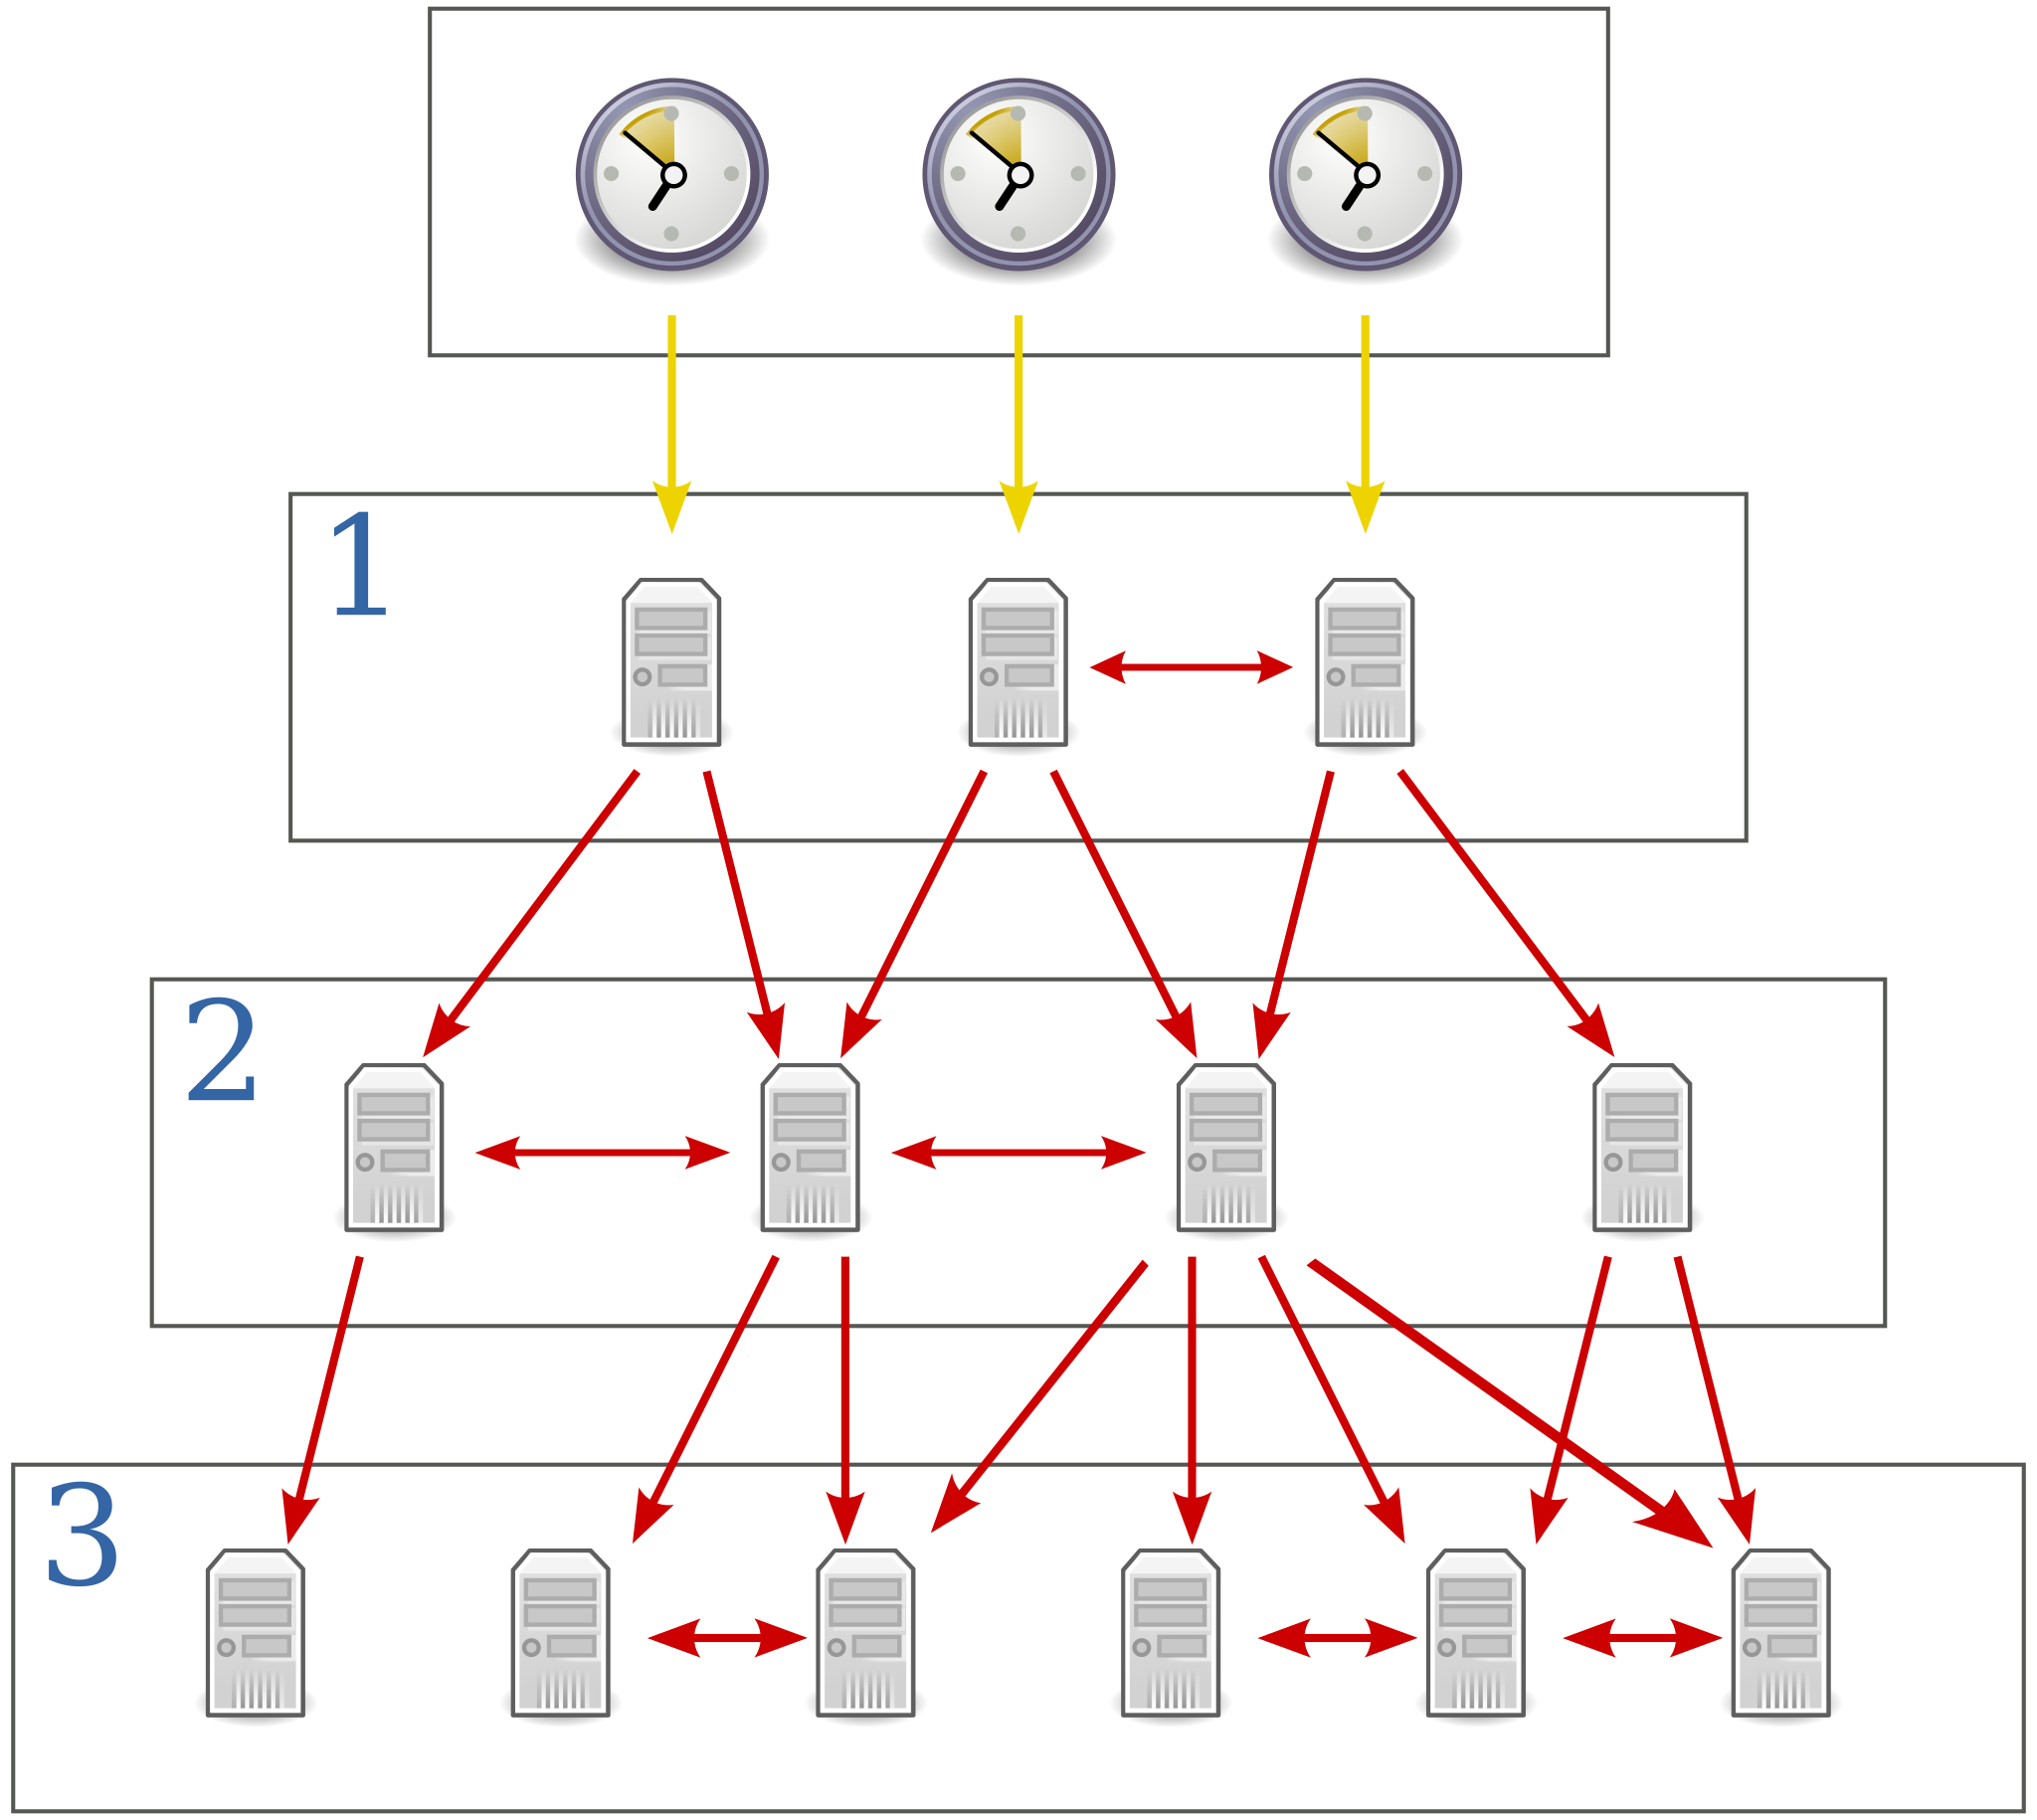
\includegraphics[width=0.7\textwidth]{figures/ntp_strata.png}
	\caption{Example of a NTP topology. The yellow arrows indicate a direct connection and the red ones a network connection.}
	\label{fig:ntp_strata}
	% https://upload.wikimedia.org/wikipedia/commons/c/c9/Network_Time_Protocol_servers_and_clients.svg
\end{figure}

NTP has a hierarchical structure of time sources. The different levels are called "stratum" and have a number from 0 to 16 assigned. This number represents the distance to the reference clock and is also used to prevent cyclical dependencies. The stratum should not be confused with the quality of the clock since this is not always true. There are stratum 3 servers providing higher quality than stratum 2 servers caused by lower latency for example. Stratum 16 indicates a unsynchronized device.

Stratum 0 devices are high-precision clocks, like atomic, GPS or other radio clocks. Usually they generate a pulse per second signal, which interrupts a connected computer to pickup the timestamp. Stratum 0 is also known as the reference clock.

Stratum 1 devices are computers which are synchronized to a stratum 0 device within microseconds. They maybe also connected to other stratum 1 servers for backup and sanity checking.

Figure \ref{fig:ntp_strata} shows an example of a logical NTP topology.

\subsection{Timestamps}

The NTP timestamp is 64 bits long and consists of a 32 bit seconds and a 32 bit fractional seconds part. That means it can represent about 136 years divided by a step size of about 233 picoseconds. NTP’s zero in time is January 1, 1900 at 00:00:00 UTC, therefore the first roll will be on February 7, 2036.

Future versions of NTP may bring a 128 bit timestamp, with a 64 bit seconds and a 64 bit fractional seconds part. NTP inventor Mills said "the 64 bit value for the fraction is enough to resolve the amount of time it takes a photon to pass an electron at the speed of light. The 64 bit second value is enough to provide unambiguous time representation until the universe goes dim".

\subsection{Algorithm}

\begin{figure}[tb]
	\centering
	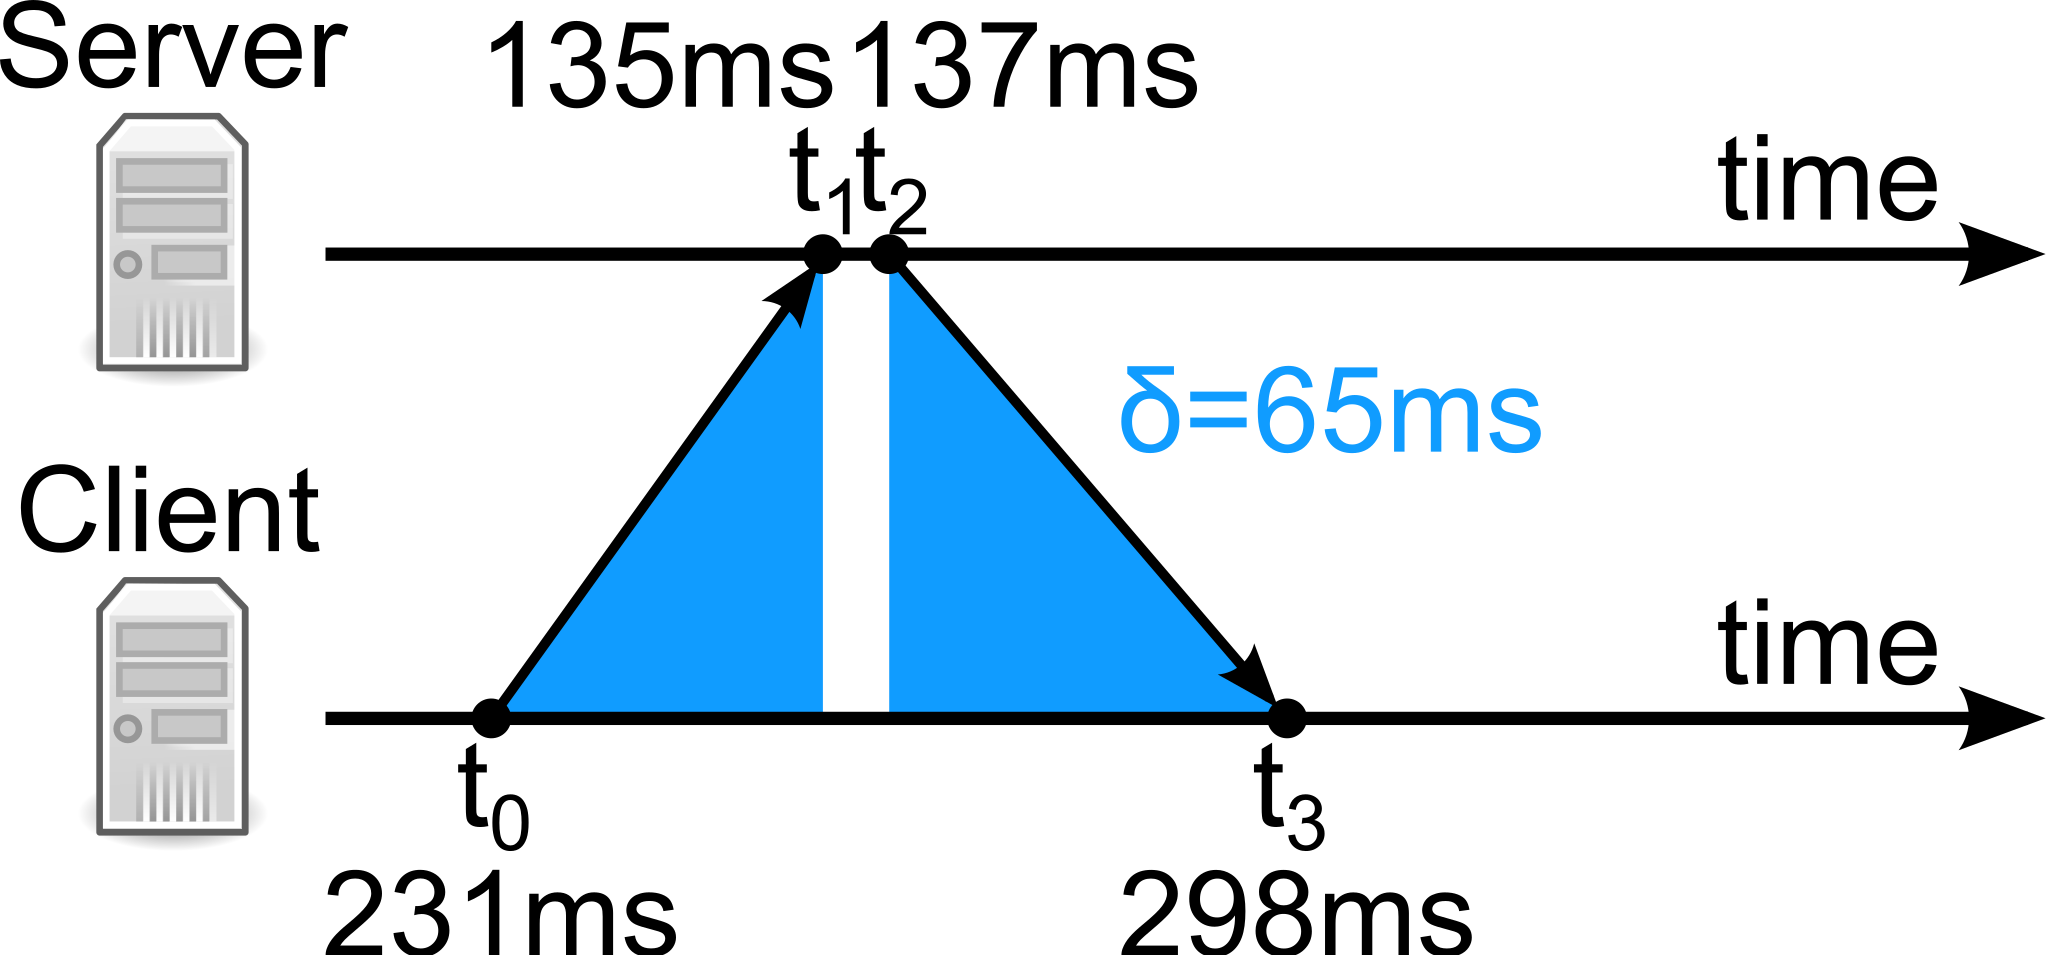
\includegraphics[width=0.7\textwidth]{figures/ntp_algorithm.png}
	\caption{Measurement process of the different timestamps}
	\label{fig:ntp_algorithm}
	% https://upload.wikimedia.org/wikipedia/commons/8/8d/NTP-Algorithm.svg
\end{figure}

With NTP the client has the full control of the synchronization process. It can poll different servers on diverse networks to synchronize its clock. As we can see in Figure \ref{fig:ntp_algorithm}, the client has 4 timestamps after such a poll. He can then calculate the time offset θ and the round-trip delay δ.

\[ \theta = \frac{(t_1 - t_0) + (t_2 - t_3)}{2} \]
\[ \delta = (t_3 - t_0) - (t_2 - t_1) \]

With:
\begin{description}
    \item[t_0] as the client's timestamp of the request packet transmission
    \item[t_1] as the server's timestamp of the request packet reception
    \item[t_2] as the server's timestamp of the response packet transmission
    \item[t_3] as the client's timestamp of the response packet reception
\end{description}

After the measurement, θ and δ are passed through filters. They are subjected to statistical analysis, outliers are discarded and the time offset is estimated. A feedback loop adjusts the clock frequency to reduce the offset gradually.

The algorithm assumes that both incoming and outgoing routes for server and client are symmetrical in regard to their delay. If this is not the case, there will be a systematic error of half the difference between client-server and server-client transmission delay.

\section{Precision Time Protocol}

Like NTP, the Precision Time Protocol (PTP) is used to synchronize clocks over packet-switched networks. But PTP promises higher clock accuracy, like sub-microsecond range on LANs. It was published 2002 in the IEEE 1588-2002 standard with the name "Standard for a Precision Clock Synchronization Protocol for Networked Measurement and Control System". The title already suggests that it could fit the needs of "Public Devices" very well. Later in 2008 the improved version PTP V2 was released in IEEE 1588-2008 which is backward compatible and improves accuracy, precision and robustness.

"IEEE 1588 is designed to fill a niche not well served by either of the two dominant protocols, NTP and GPS. IEEE 1588 is designed for local systems requiring accuracy beyond those attainable using NTP. It is also designed for applications that cannot bear the cost of a GPS receiver at each node, or for which GPS signals are inaccessible."

\section{Algorithm}

% figure

The master periodically broadcasts his current time $t_1$ as a \textit{Sync} message to the slaves. Under IEEE 1588-2002 broadcasts are up to once per second. Under IEEE 1588-2008, up to 10 per second are permitted. The slaves record the timestamp $t_2$ on receiving the \textit{Sync} message.

The \textit{Follow\_Up} message is optionally. Not all masters have the ability to provide an accurate timestamp right at sending the \textit{Sync} message. With common hardware and OS the best estimation of $t_1$ is right after the transmission is complete. This limitation leads the master to send the \textit{Follow\_Up} message to propagate $t_1$.

The slave continues with a \textit{Delay\_Req} message and keeps the transmission timestamp $t_3$. This is necessary to measure the individual round-trip time and to accurately synchronize to the master. After receiving the \textit{Delay\_Req} message and taking the timestamp $t_4$, the master responds with a \textit{Delay\_Resp} message and $t_4$.

After this procedure the slave has recorded the timestamps $t_1$, $t_2$, $t_3$ and $t_4$ which are necessary for calculating the offset from the master.

\[ o = \frac{(t_2 - t_1) + (t_3 - t_4)}{2} \]

The offset is then used to correct the slave by this amount to bring it into agreement with their master.

Like NTP, the offset and timestamps can further be passed through filters and subjected to statistical analysis. A feedback loop adjusts the clock frequency to reduce the offset gradually.

A few assumptions are made. First, the exchange of messages happens so fast that the measured offset can be considered as constant in between. Another assumption is, like with NTP, that the exchange has a symmetrical delay in both directions. Finally, it is assumed that timestamps can be measured accurately on sending and receiving messages. The resulting accuracy of PTP depends on how true these assumptions are in reality.

\section{Global Positioning System}

The Global Positioning System (GPS) is a global navigation satellite system (GNSS) set up to provide location and time information all around the world under all weather conditions. To do so, it needs an unobstructed line of sight to four or more GPS satellites. It has no further dependencies of any cellular or internet connection, but can be enhanced by those. The system was created by the US government, which maintains it and makes it freely accessible to anyone.

Each satellite transmits its position and time to the earth. A GPS device that receives messages from at least 4 different satellites is able to calculate its position.

As GPS is very time sensitive, each satellite carries a very stable atomic clock which is synchronized with another one and ground clocks. The clock drift is corrected every day.
These very accurate clocks can be used to synchronize a computer’s clock within nanoseconds.

